%%%%%%%%%%%%%%%%%%%%%%%%%%%%%%%%%%%%%%%%%%%%%%%%%%%%%%%%%%%%%%%%%%%%%%%%%%%%%%%
\documentclass[hyperref={pdfpagelabels=false},compress,table]{beamer} % 在Mac下无法编译
% \documentclass[compress,table]{beamer} % 在Mac下使用
% package for font
\usepackage{fontspec}
\defaultfontfeatures{Mapping=tex-text}  %%如果没有它,会有一些 tex 特殊字符无法正常使用,比如连字符。
\usepackage{xunicode,xltxtra}
\usepackage[BoldFont,SlantFont,CJKnumber,CJKchecksingle]{xeCJK}  % \CJKnumber{12345}: 一万二千三百四十五
\usepackage{CJKfntef}  %%实现对汉字加点、下划线等。
\usepackage{pifont}  % \ding{}
% package for math
\usepackage{amsfonts}

% package for graphics
\usepackage[americaninductors,europeanresistors]{circuitikz}
\usepackage{tikz}
\usetikzlibrary{plotmarks}  % placements=positioning
\usepackage{graphicx}  % \includegraphics[]{}
\usepackage{subfigure}  %%图形或表格并排排列
% package for table
\usepackage{colortbl,dcolumn}  %% 彩色表格
\usepackage{multirow}
\usepackage{multicol}
\usepackage{booktabs}
% package for code
\usepackage{fancyvrb}
\usepackage{listings}

% \usepackage{animate}
% \usepackage{movie15}

%%%%%
% setting for beamer
\usetheme{default} % Madrid(常用), Copenhagen, AnnArbor, boxes(白色), Frankfurt,Berkeley
\useoutertheme[subsection=true]{miniframes} % 使用Berkeley时注释本行
\usecolortheme{sidebartab}
\usefonttheme{serif}  %%英文使用衬线字体
% \setbeamertemplate{background canvas}[vertical
% shading][bottom=white,top=structure.fg!7] %%背景色,上25%的蓝,过渡到下白。
\setbeamertemplate{theorems}[numbered]
\setbeamertemplate{navigation symbols}{}  %% 去掉页面下方默认的导航条
\setbeamercovered{transparent}  %设置 beamer 覆盖效果

% 设置标题title背景色
% \setbeamercolor{title}{fg=black, bg=lightgray!60!white}
\setbeamercolor{title}{fg=white, bg=black!70!white}

% 设置每页小LOGO
\pgfdeclareimage[width=1cm]{ouc}{figures/static/ouc.pdf}
\logo{\pgfuseimage{ouc}{\vspace{-20pt}}}

% setting for font
%%\setCJKmainfont{Adobe Kaiti Std}
\setCJKmainfont{SimSun} 
%% \setCJKmainfont{FangSong_GB2312} 
%% \setmainfont{Apple Garamond}  %%苹果字体没有SmallCaps
\setCJKmainfont{SimSun} 
%FUNNY%\setCJKmainfont{DFPShaoNvW5-GB}  %%华康少女文字W5(P)
%FUNNY%\setCJKmainfont{FZJingLeiS-R-GB}  %%方正静蕾体
%FUNNY%\setmainfont{Purisa}
%\setsansfont[Mapping=tex-text]{Adobe Song Std}
     %如果装了Adobe Acrobat,可在font.conf中配置Adobe字体的路径以使用其中文字体。
     %也可直接使用系统中的中文字体如SimSun、SimHei、微软雅黑等。
     %原来beamer用的字体是sans family;注意Mapping的大小写,不能写错。
     %设置字体时也可以直接用字体名,以下三种方式等同:
     %\setromanfont[BoldFont={黑体}]{宋体}
     %\setromanfont[BoldFont={SimHei}]{SimSun}
     %\setromanfont[BoldFont={"[simhei.ttf]"}]{"[simsun.ttc]"}
% setting for graphics
\graphicspath{{figures/}}  %%图片路径
\renewcommand\figurename{图}

% setting for pdf
\hypersetup{% pdfpagemode=FullScreen,%
            pdfauthor={Xiaodong Wang},%
            pdftitle={Title},%
            CJKbookmarks=true,%
            bookmarksnumbered=true,%
            bookmarksopen=false,%
            plainpages=false,%
            colorlinks=true,%
            citecolor=green,%
            filecolor=magenta,%
            linkcolor=blue,%red(default)
            urlcolor=cyan}

% setting for fontspec
\XeTeXlinebreaklocale "zh"  %%表示用中文的断行
\XeTeXlinebreakskip = 0pt plus 1pt minus 0.1pt  %%多一点调整的空间
%%%%%

% font setting by xeCJK
\setCJKfamilyfont{NSimSun}{NSimSun}
\newcommand{\song}{\CJKfamily{NSimSun}}
%%%\setCJKfamilyfont{AdobeSongStd}{Adobe Song Std}
%%%\newcommand{\AdobeSong}{\CJKfamily{AdobeSongStd}}
\setCJKfamilyfont{FangSong}{FangSong_GB2312}
\newcommand{\fang}{\CJKfamily{FangSong}}
%%%\setCJKfamilyfont{AdobeFangsongStd}{Adobe Fangsong Std}
%%%\newcommand{\AdobeFang}{\CJKfamily{AdobeFangsongStd}}
\setCJKfamilyfont{SimHei}{SimHei}
\newcommand{\hei}{\CJKfamily{SimHei}}
%%%\setCJKfamilyfont{AdobeHeitiStd}{Adobe Heiti Std}
%%%\newcommand{\AdobeHei}{\CJKfamily{AdobeHeitiStd}}
\setCJKfamilyfont{KaiTi}{KaiTi}
\newcommand{\kai}{\CJKfamily{KaiTi}}
%%%\setCJKfamilyfont{AdobeKaitiStd}{Adobe Kaiti Std}
\newcommand{\AdobeKai}{\CJKfamily{AdobeKaitiStd}}
\setCJKfamilyfont{LiSu}{LiSu}
\newcommand{\li}{\CJKfamily{LiSu}}
\setCJKfamilyfont{YouYuan}{YouYuan}
\newcommand{\you}{\CJKfamily{YouYuan}}
\setCJKfamilyfont{FZJingLei}{FZJingLeiS-R-GB}
\newcommand{\jinglei}{\CJKfamily{FZJingLei}}
\setCJKfamilyfont{MSYH}{Microsoft YaHei}
\newcommand{\msyh}{\CJKfamily{MSYH}}

% 自定义颜色
\def\Red{\color{red}}
\def\Green{\color{green}}
\def\Blue{\color{blue}}
\def\Mage{\color{magenta}}
\def\Cyan{\color{cyan}}
\def\Brown{\color{brown}}
\def\White{\color{white}}
\def\Black{\color{black}}

\lstnewenvironment{xmlCode}[1][]{% for Java
  \lstset{
    basicstyle=\tiny\ttfamily,%
    columns=flexible,%
    framexleftmargin=.7mm, %
    % frame=shadowbox,%
    % rulesepcolor=\color{cyan},%
     frame=single,%
    backgroundcolor=\color{white},%
    xleftmargin=4\fboxsep,%
    xrightmargin=4\fboxsep,%
    numbers=left,numberstyle=\tiny,%
    numberblanklines=false,numbersep=7pt,%
    language=xml, %
    }\lstset{#1}}{}

\lstnewenvironment{javaCode}[1][]{% for Java
  \lstset{
    basicstyle=\tiny\ttfamily,%
    columns=flexible,%
    framexleftmargin=.7mm, %
    frame=shadowbox,%
    rulesepcolor=\color{cyan},%
    % frame=single,%
    backgroundcolor=\color{white},%
    xleftmargin=4\fboxsep,%
    xrightmargin=4\fboxsep,%
    numbers=left,numberstyle=\tiny,%
    numberblanklines=false,numbersep=7pt,%
    language=Java, %
    }\lstset{#1}}{}

\lstnewenvironment{shCode}[1][]{% for Java
  \lstset{
    basicstyle=\scriptsize\ttfamily,%
    columns=flexible,%
    framexleftmargin=.7mm, %
    frame=shadowbox,%
    rulesepcolor=\color{brown},%
    % frame=single,%
    backgroundcolor=\color{white},%
    xleftmargin=4\fboxsep,%
    xrightmargin=4\fboxsep,%
    numbers=left,numberstyle=\tiny,%
    numberblanklines=false,numbersep=7pt,%
    language=sh, %
    }\lstset{#1}}{}

\newcommand\ask[1]{\vskip 4bp \tikz \node[rectangle,rounded corners,minimum size=6mm,
  fill=white,]{\Cyan \includegraphics[height=1.5cm]{question} \Large \msyh #1};}

\newcommand\wxd[1]{\vskip 4bp \tikz \node[rectangle,minimum size=6mm,
  fill=blue!60!white,]{\White \ding{118} \msyh #1};}

\newcommand\xyy[1]{\vskip 2bp \tikz \node[rectangle,minimum size=3mm,
  fill=black!80!white,]{\White \msyh\scriptsize #1};}

\newcommand\cxf[1]{\vskip 4bp \tikz \node[rectangle,rounded corners,minimum size=6mm,
  fill=orange!60!white,]{\White \ding{42} \msyh #1};}

\newcommand\samp[1]{\vskip 2bp \tikz \node[rectangle,minimum size=3mm,
  fill=white!100!white,]{\Mage\msyh \small CODE \ding{231} \Black #1};\vskip -8bp}

\newcommand\zhyfly[1]{\tikz \node[rectangle,rounded corners,minimum size=6mm,ball color=red!25!blue,text=white,]{#1};}

\setbeamerfont{frametitle}{series=\msyh} % 修改Beamer标题字体

\makeatletter
\newcommand{\Extend}[5]{\ext@arrow 0099{\arrowfill@#1#2#3}{#4}{#5}}
\makeatother


%%%%%%%%%%%%%%%%%%%%%%%%%%%%%%%%%%%%%%%%%%%%%%%%%%%%%%%%%%%%%%%%%%%%%%%%%%%%%%%
% \titlepage
\title[KevinW@OUC]{\hei {\huge Java EE企业应用系统设计}\\  
HTTP请求处理编程}
\author[王晓东]{王晓东\\
  \href{mailto:wangxiaodong@ouc.edu.cn}{\footnotesize wangxiaodong@ouc.edu.cn}}
\institute[中国海洋大学]{\small 中国海洋大学}
\date{\today}
\titlegraphic{\vspace{-6em}
\includegraphics[height=6cm]{static/ouc.pdf}\vspace{-6em}}
%%%%%
\begin{document}
%% Delete this, if you do not want the table of contents to pop up at
%% the beginning of each subsection:
\AtBeginSection[]{                              % 在每个Section前都会加入的Frame
  \frame<handout:0>{
    \frametitle{\textbf{\hei 接下来…}}
    \tableofcontents[currentsection]
  }
}  %

\AtBeginSubsection[]                            % 在每个子段落之前
{
  \frame<handout:0>                             % handout:0 表示只在手稿中出现
  {
    \frametitle{\textit{\hei 接下来…}}\small
    \tableofcontents[current,currentsubsection] % 显示在目录中加亮的当前章节
  }
}
 \frame{\titlepage}

%%%%%%%%%%%%%%%%%%%%%%%%%%%%%%%%%%%%%%%%%%%%%%%%
\begin{frame}
\frametitle{参考书目}
\begin{enumerate}
\item 吕海东,张坤 编著,Java EE企业级应用开发实例教程,清华大学出版社,2010年8月
\end{enumerate}  
\end{frame}

% \begin{frame}
% \frametitle{本章学习目标}
% \begin{enumerate}
% \item 
% \end{enumerate}  
% \end{frame}

\section*{大纲}
\frame{\frametitle{大纲} \tableofcontents}

\section{HTTP请求内容}

\begin{frame}[fragile] % [fragile]参数使得能够插入代码
\frametitle{Web工作模式} 
\begin{itemize}\kai
\item Web使用请求-响应模式。
\item 客户端(浏览器)向服务器发出HTTP请求。
\item 在HTTP请求中包含传递到服务器的数据。
\item Web服务器接收到请求,对请求进行处理。
\item Web服务器通过HTTP向客户端发送响应。
\item 客户端接收到响应后,进行显示或跳转。
\end{itemize}
\end{frame}

\begin{frame}[fragile,fragile] % [fragile]参数使得能够插入代码
\frametitle{HTTP请求中包含的信息} 

HTTP请求中包含的信息包括请求头和请求体。

\wxd{请求头}

{\small
\begin{verbatim}
GET /articles/news/today.jsp HTTP/1.1 
Accept: */*
Accept-Language: en-us 
Connection: Keep-Alive 
Host: localhost
Referer: http://localhost/links.asp
User-Agent: Mozilla/4.0 (compatible; MSIE 5.5; Windows NT 5.0)
Accept-Encoding:gzip, deflate
... 
\end{verbatim}
}
\end{frame}

\begin{frame}[fragile] % [fragile]参数使得能够插入代码
\frametitle{HTTP请求中包含的信息} 

\xyy{http请求头标记和说明}
\begin{description}\kai
\item[User-Agent] 浏览器的机器环境。
\item[Accept] 浏览器支持哪些MIME数据类型。
\item[Accept-Charset] 浏览器支持的字符编码。
\item[Accept-Encoding] 浏览器支持哪种数据压缩格式。
\item[Accept-Language] 浏览器指定的语言环境。
\item[Host] 浏览器访问的主机名。
\item[Referer] 浏览器是从哪个页面来的。
\item[Cookie] 浏览器保存的cookie对象。
\end{description}

Java EE Web组件Servlet和JSP中可以使用请求对象的方法读取这些请求内容,进而进行相应的处理。

\end{frame}

\begin{frame}[fragile,fragile] % [fragile]参数使得能够插入代码
\frametitle{HTTP请求中包含的信息} 
\wxd{请求体} 

每次HTTP请求时,在请求头之后会有一个空行,接下来是请求中包含的提交数据,即请求体。

\xyy{GET请求}

请求数据直接在请求的URL地址中,作为URL的一部分发送给Web服务器。
\begin{verbatim}
http://localhost:8080/web01/login.do?id=9001&pass=9001
\end{verbatim}
请求体为空,提交数据直接在URL上,作为请求头部分传输到Web服务器,通过URL的QueryString部分能得到提交的参数数据。

此种方式对提交数据的大小有限制,不同浏览器会有所不同,如IE为2083字节。GET请求时数据会出现在URL中,保密性差,实际编程中要尽量避免。
\end{frame}

\begin{frame}[fragile,fragile] % [fragile]参数使得能够插入代码
\frametitle{HTTP请求中包含的信息} 

\xyy{POST请求}

请求体数据单独打包为数据块,通过Socket直接传递到Web服务器端,数据不会在地址栏出现。可以提交大的数据,包括二进制文件,实现文件上传功能。原则上POST请求对提交的数据没有大小限制。
\end{frame}

\section{Java EE请求对象}

\begin{frame}
\frametitle{请求对象类型与生命周期} 
\wxd{请求对象接口类型}
\begin{itemize}
\item Java EE规范中的通用请求对象要实现接口javax.servlet.ServeltRequest
\item HTTP请求对象要实现接口javax.servlet.http.HttpServletRequest
\end{itemize}

\wxd{请求对象生命周期}

在Java Web组件开发中,不需要Servlet或JSP自己创建请求对象,它们由Web容器自动创建,并传递给Servlet和JSP的服务方法doGet和doPost,在服务处理方法中直接使用请求对象即可。
\end{frame}

\begin{frame}
\frametitle{请求对象类型与生命周期} 
\wxd{请求对象创建}

每次Web服务器接收到HTTP请求时,会自动创建实现HttpServletRequest接口的对象。在创建该对象之后,Web服务器将请求头和请求体信息写入请求对象,Servlet和JSP可以通过请求对象的方法取得这些请求信息,继而可以取得用户提交的数据。

\wxd{请求对象销毁}

当Web服务器处理HTTP请求,向客户端发送HTTP响应结束后,会自动销毁请求对象,保存在请求对象中的数据随即丢失。当下次请求时新的请求对象又会被创建。
\end{frame}

\begin{frame}[fragile] % [fragile]参数使得能够插入代码
\frametitle{请求对象功能与方法} 

请求对象方法一般分类为:
\begin{itemize}
\item 取得请求头信息。
\item 取得请求体中包含的提交参数数据,包含表单元素或地址栏URL的参数。
\item 取得客户端的有关信息,如请求协议、IP地址和端口等。
\item 取得服务器端的相关信息,如服务器的IP等。
\item 取得请求对象的属性信息,用于在一个请求的转发对象之间传递数据。
\end{itemize}
\end{frame}

\begin{frame}[fragile] % [fragile]参数使得能够插入代码
\frametitle{取得请求头方法} 

\begin{itemize}
\item String getHeader(String name)
\begin{javaCode}
String browser = request.getHeader("User-Agent");
\end{javaCode}

\item int getIntHeader(String name)
\begin{javaCode}
int size = request.getIntHeader("Content-Length");
\end{javaCode}

\item long getDateHeader(String name)
\begin{javaCode}
long datetime = request.getDateHeader("If-Modified-Since");
\end{javaCode}

\item Enumeration getHeaderNames()
\begin{javaCode}
for (Enumeration enume = reqeust.getHeaderNames(); enum.hasMoreElements(); ) {
  String headerName = (String) enume.nextElement();
  System.out.println("Name = " + headerName);
}
\end{javaCode}
\end{itemize}
\end{frame}

\begin{frame}[fragile,fragile] % [fragile]参数使得能够插入代码
\frametitle{取得请求中包含的提交参数数据} 

在Web开发中,用户通过表单输入将客户段数据提交到服务器端,这些数据被Web服务器自动保存到请求对象中。Web组件Servlet和JSP可以通过请求对象获得用户提交的数据。

\wxd{String getParameter(String name)} 取得指定名称的参数数据。

参数name为FORM表单元素的name或URL参数名称:
\begin{verbatim}
产品名称:<input type="text" name="productName" />
productSearch.do?productName=Acer
\end{verbatim}

如下代码可以取得以上的参数名为productName的数据:
\begin{javaCode}
String productName = request.getParameter("productName");
\end{javaCode}
\end{frame}

\begin{frame}[fragile,fragile] % [fragile]参数使得能够插入代码
\frametitle{取得请求中包含的提交参数数据} 

\wxd{String[] getParameterValues(String name)} 取得指定名称的参数数据数组,如复选框和复选列表。

如下代码取得复选框的选择数据:
\begin{verbatim}
爱好:
<input type="checkbox" name="behave" value="旅游">旅游
<input type="checkbox" name="behave" value="读书">读书
<input type="checkbox" name="behave" value="体育">体育
\end{verbatim}

如下代码取得选定的爱好:

\begin{javaCode}
String[] behaves = request.getParameterValues("behave");
for (int i = 0; i < behaves.length; i++) {
  out.println(behaves[i]);
}
\end{javaCode}
\end{frame}

\begin{frame}[fragile] % [fragile]参数使得能够插入代码
\frametitle{取得请求中包含的提交参数数据} 
\wxd{Enumeration getParameterNames()} 取得所有请求的参数名称。

\begin{javaCode}
for (Enumeration enums = request.getParameterNames(); enums.hasMoreElements();) {
  String paramName = (String) enums.nextElement();
  System.out.println(paramName);
}
\end{javaCode}
\end{frame}

\begin{frame}[fragile] % [fragile]参数使得能够插入代码
\frametitle{取得请求中包含的提交参数数据} 

\wxd{Map getParameterMap()} 取得所有请求的参数名和值,包装在一个Map对象中,可以使用这个对象同时取得所有的参数名和参数值。

\begin{javaCode}
Map params = request.getParameterMap();
Set names = params.keySet();
for (Object o: names) {
  String paramName = (String) o;
  out.print(paramName + " = " + params.get(paramName) + "<br/>");
}
\end{javaCode}
\end{frame}

\begin{frame}[fragile] % [fragile]参数使得能够插入代码
\frametitle{取得请求中包含的提交参数数据} 

在Web开发中,用户通过表单输入将客户段数据提交到服务器端,这些数据被Web服务器自动保存到请求对象中。Web组件Servlet和JSP可以通过请求对象获得用户提交的数据。

\wxd{Map getParameterMap()} 取得所有请求的参数名和值,包装在一个Map对象中。
\begin{javaCode}
Map params = request.getParameterMap();
Set names = params.keySet();
for (Object o: names) {
  String paramName = (String) o;
  out.println(paramName + " = " + params.get(paramName) + "<br/>");
}
\end{javaCode}
\end{frame}

\begin{frame}[fragile,fragile] % [fragile]参数使得能够插入代码
\frametitle{取得请求中包含的提交参数数据} 

\wxd{ServletInputStream getInputStream() throws IOException} 取得客户端的输入流。

当使用getParameter()方法后,就无法使用getInputStream()方法,反之亦然。

当用户提交的数据中包含文件上传时,提交的数据就可以以二进制编码方式提交到服务器。当表单既有文本字段还有文件上传时,就需要对此二进制流进行解析,从而分离出文本和上传文件。可以使用第三方框架实现上传文件的大额处理,如Apache的Common upload组件。

\begin{verbatim}
<form action="" method="" enctype="multipart/form-data" />
姓名:<input type="text" name="name" /><br />
照片:<input type="file" name="photo" /><br />
<input type="submit" value="提交" />
</form>
\end{verbatim}
\end{frame}

\begin{frame}[fragile] % [fragile]参数使得能够插入代码
\frametitle{取得其他客户端信息} 

\wxd{String getRemoteHost()}

取得请求客户的主机名。

\wxd{String getRemoteAddr()}

取得请求客户端的IP地址。

\wxd{int getRemotePort()}

取得请求客户的端口号。

\wxd{String getProtocol()}

取得请求的协议。
\end{frame}

\begin{frame}[fragile] % [fragile]参数使得能够插入代码
\frametitle{取得其他客户端信息} 

\wxd{String getContentType()}

取得请求体的内容类型,以MIME表达。

\wxd{int getContentLength()}

取得请求体为二进制流时请求体的长度,一般当处理文件上传时使用。

\wxd{String getProtocol()}

取得请求的协议,一般为HTTP,返回HTTP1.1。
\end{frame}

\begin{frame}[fragile] % [fragile]参数使得能够插入代码
\frametitle{取得服务器端信息} 

\wxd{String getServerName()}

取得服务器的HOST,一般为IP地址。

\wxd{int getServerPort()}

取得服务器接收端口。
\end{frame}

\begin{frame}[fragile] % [fragile]参数使得能够插入代码
\frametitle{应用实例} 

\wxd{EE\_4.3 取得HTML表单提交的数据}
\end{frame}
%%%%%%%%%%%%%%%%%%%%%%%%%%
\begin{frame}[fragile] % [fragile]参数使得能够插入代码
\frametitle{} 

\end{frame}
%%%%%%%%%%%%%%%%%%%%%%%%%%
%% \begin{figure}
%% \centering
%% 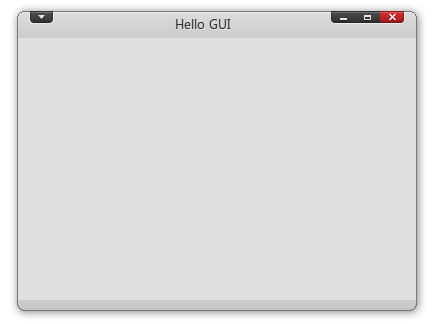
\includegraphics[width=0.6\textwidth]{fig01.png}
%% \end{figure}
% TKS %%%%%%%%%%%%%%%%%%%%%%%%%%%%%%%%%%%%%%%%%%%%%%
\begin{frame}
\centering
{\Huge \textcolor{blue}{THE END}} \\
\vspace{5mm}
{\Large wangxiaodong@ouc.edu.cn} \\
\end{frame}
%%%%%%%%%%%%%%%%%%%%%%%%%%%%%%%%%%%%%%%%%%%%%%%%%%
\end{document}
